\section{Results and Discussion}

To look at the effects of the demand on the output, the demand data is scaled up and down to allow a comparison between high-use years and low-use years. Similarly, sensitivity analysis is performed on the location, to see how important the location can be on the performance.

\subsection{Case 1: Scotland }

Case 1 uses the Lord Thomson building at Heriot-Watt University as the demand. The resource data used is for Edinburgh, Scotland. Three scenarios are simulated which include the base case, where the demand is unchanged, a reduced demand scenario, where the demand is reduced by 50\% and a third scenario where the demand is reduced by 90\%. 

\subsubsection{Pareto Front}

\begin{figure}[H]
	\centering
    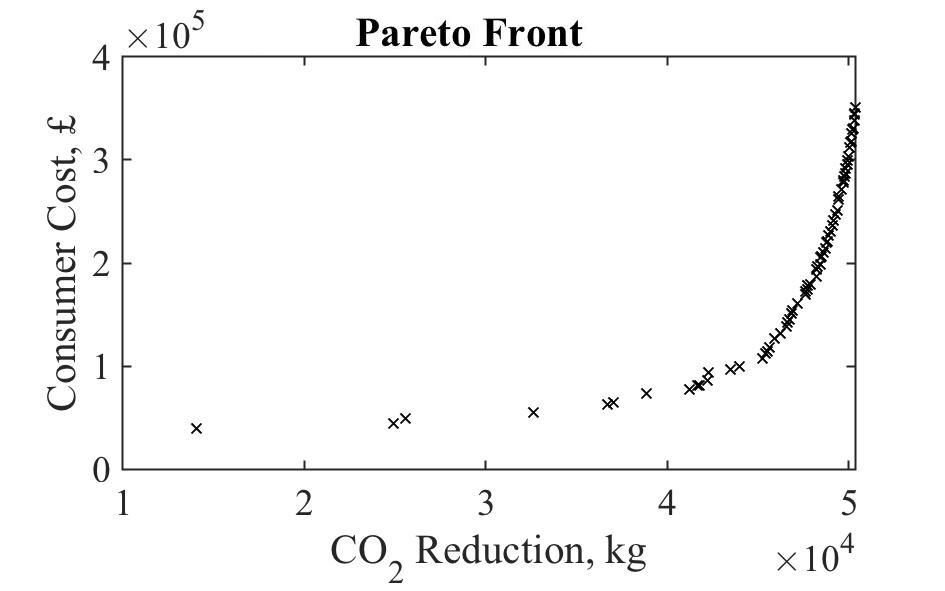
\includegraphics[width=\columnwidth]{Figures/ParetoBase.jpg}
    \caption{The Pareto front for the base case scenario. The two optimised objective functions are plotted with consumer cost on the y-axis and $co_2$ reduction on the x-axis.}
    \label{fig:ParetoBase}
\end{figure}

Fig. \ref{fig:ParetoBase} shows the pareto front obtained from the simulation. It shows a trend of increased CO$_2$ reduction leading to an increase in the consumer cost. The consumer cost is being minimised while the CO$_2$ reduction is being maximised. The range of solutions is from £50,000 to £440,000 for consumer cost. The CO$_2$ reduction ranges from approximately 15,000 kg to 50,000 kg. This is the base case pareto front, where it is not possible to get anywhere near meeting the demand. In this case the constraint on the minimum acceptable solution is not set. This is due to two factors: The first being a high demand for the building; The second is the low strength of the solar insolation coupled with the lack of roof space required at that strength. When a value is set for the constraint, the simulation cannot run.

\begin{table}[H]
\caption{Four selected solutions on the Pareto front ranging from minimum to maximum points for Case 1.}
\vspace{5pt}
\label{case1}
\centering
\begin{tabular}{@{}llll@{}}
\toprule
\begin{tabular}{@{}l@{}}{\textbf{CO$_2$}} \\ \textbf{Reduction, kg}\end{tabular} 
& \begin{tabular}{@{}l@{}}{\textbf{Consumer}} \\ \textbf{Cost, £}\end{tabular} 
& \begin{tabular}{@{}l@{}}{\textbf{PV/ST}}  \\ \textbf{Panels}\end{tabular}
& \begin{tabular}{@{}l@{}}{\textbf{Li-ion/Heat}} \\ \textbf{Batteries}\end{tabular} \\ \toprule
50,000 & 351,000 & 517/245 & 46/27 \\ \midrule
48,000 & 161,000 & 708/80 & 29/7 \\ \midrule
37,000 & 63,000 & 494/8 & 14/4 \\ \midrule
14,000 & 40,000 & 101/20 & 1/8 \\ \midrule
\end{tabular}
\end{table}

Table \ref{case1} gives four selected solutions on the pareto front. These solutions are the maximum and minimum points on the front and one point at each side of the curve. The values vary greatly, but all lie on the pareto front and therefore are classed as pareto optimal solutions.



\subsubsection{Optimised Objectives vs Simulation Variables}

\begin{figure}[H]
	\centering
    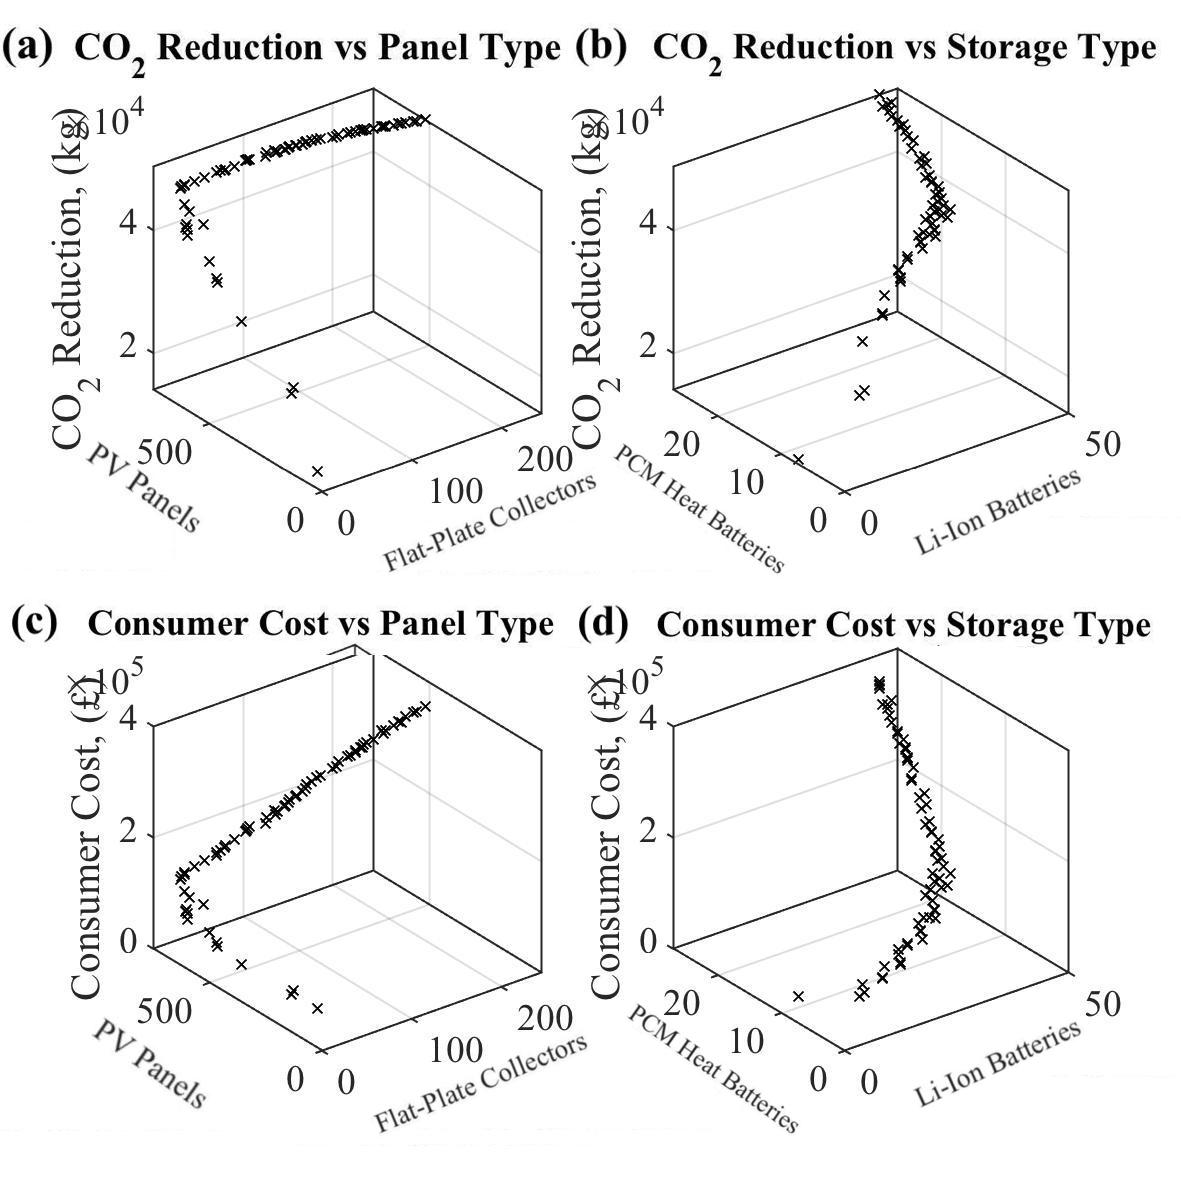
\includegraphics[width=235pt]{Figures/RedAndCostVsPanelsAndStorageBase1.jpg}
    \caption{3-Dimensional plots of the optimised objectives with respect to the the simulation variables. (a) Panel type vs CO$_2$ reduction, (b) Storage type vs CO$_2$ reduction, (c) Panel type vs consumer cost, and (d) Storage type vs consumer cost}
    \label{fig:ObjectivesVsPanelsVsStorage}
\end{figure}
  
  Fig. \ref{fig:ObjectivesVsPanelsVsStorage} is the amount of PV and solar thermal panels used for each scenario on the Pareto front plotted against the CO$_2$ reduction. This shows that the main factor in reducing the amount of CO$_2$ produced is by increasing the number of PV panels. It increases the reduction in CO$_2$ from 30,000 kg at 300 PV panels to 45,000 kg at 800 PV panels. As the amount of flat plate collectors increases, the reduction in CO$_2$ emissions is not greatly affected. This is due to the fact that, despite a reduction of 0.24 kg CO$_2$/kWh generated, the direct solar insolation present is not strong enough to produce energy for a large portion of the year. The flat plate collectors contribute approximately 5000 kg of reduced CO$_2$ emissions at 200 collectors. Figure 3(c) shows the effect on consumer cost of the various combinations of panels. It can be seen that the flat plate collectors are a larger outlay. This is expected as due to the low amount of energy produced by each flat plate collector, the tariff (see \ref{Constants}) from generating energy is unable to have a large effect on the outlay. Whereas with PV panels, the initial outlay is offset by the tariff on generating electricity in this way. The overall consumer cost ranges from approximately £30,000 up to £400,000. Most of the solutions occur between £100,000 and £400,000 consumer cost. Fig. 3(b) and Fig. 3(d) detail the storage means with each of the objective functions. In general, the more of each type of battery in the system, the higher the cost and the higher the reduction in emissions. This is in line with the amount of each type of panel being used to generate the energy. 
  
\subsubsection{Storage Performance}

\begin{figure}[H]
	\centering
    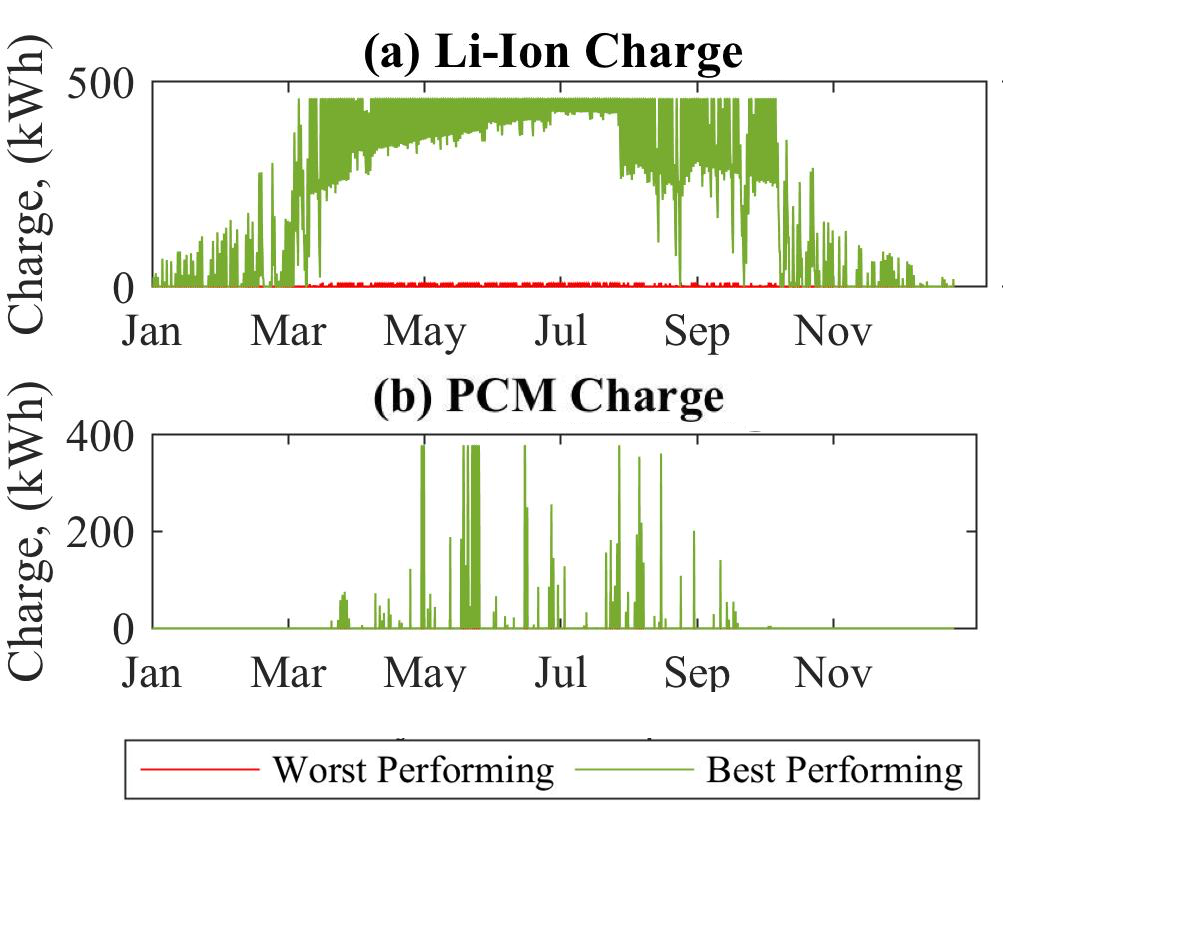
\includegraphics[width=1.1\columnwidth]{Figures/StorageLevels.png}
    \vspace*{-15mm}
    \caption{(a) Hourly charge level of the Li-Ion battery array in kWh with respect to time and (b) PCM heat battery array in kWh with respect to time.}
    \label{fig:StorageLevels}
\end{figure}
  
Fig. \ref{fig:StorageLevels}(a) shows the best and worst performing Li-Ion battery scenarios. The best-case scenario, in green, shows a maximum level of 420 kWh. It remains above zero, i.e. the demand is being met at all times from April until mid-October, apart from on two short occasions in September and October. Between January and March, and November and December the battery bank level depletes to zero on numerous occasions. This indicates that not enough energy is being produced to meet the demand. This is also the circumstance for the worst case, shown in red. The worst case is unable to provide any energy to meet the demand outwith the months of March to October.
 
In the case of the best and worst performing scenarios for the PCM heat battery, shown in Fig. \ref{fig:StorageLevels}(b), the worst performing scenario results in zero kWh of thermal energy being stored at any point. The best performance is still inadequate. This is due to the poor direct insolation at the location. The maximum level of the battery bank is only reached on very few occasions during the year and each time it reaches maximum capacity, the stored energy is then utilised soon after in order to meet the demand.

\begin{figure}[H]
	\centering
    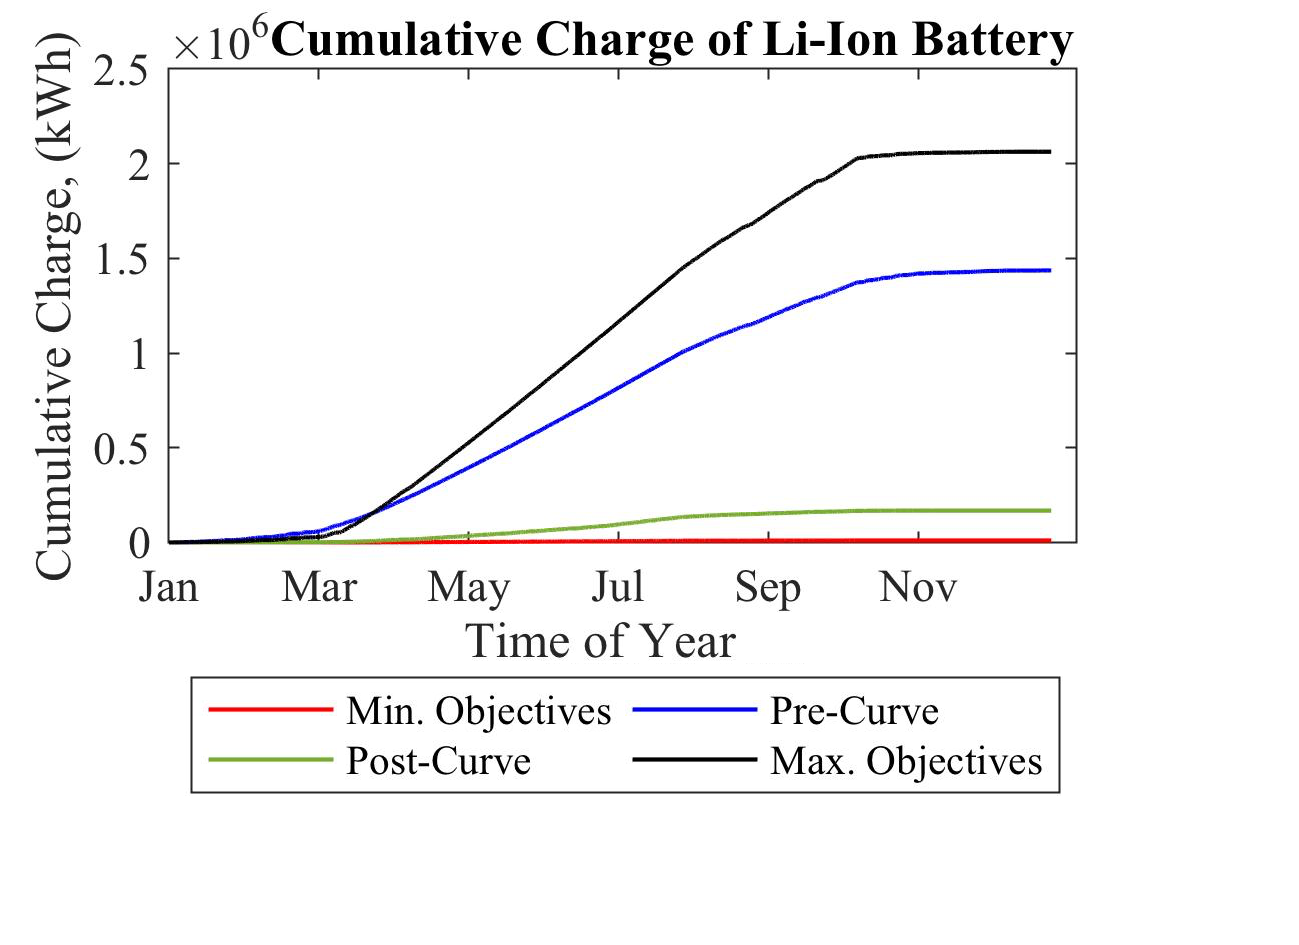
\includegraphics[width=255pt]{Figures/CumChargeBat.png}
    \vspace*{-15mm}
    \caption{Four scenarios for the cumulative charge of the Li-Ion battery array with respect to time. Each line represents one point on the Pareto front from lowest consumer cost to highest consumer cost.}
    \label{fig:CumChargeBat}
\end{figure}
 
 \begin{figure}[H]
	\centering
    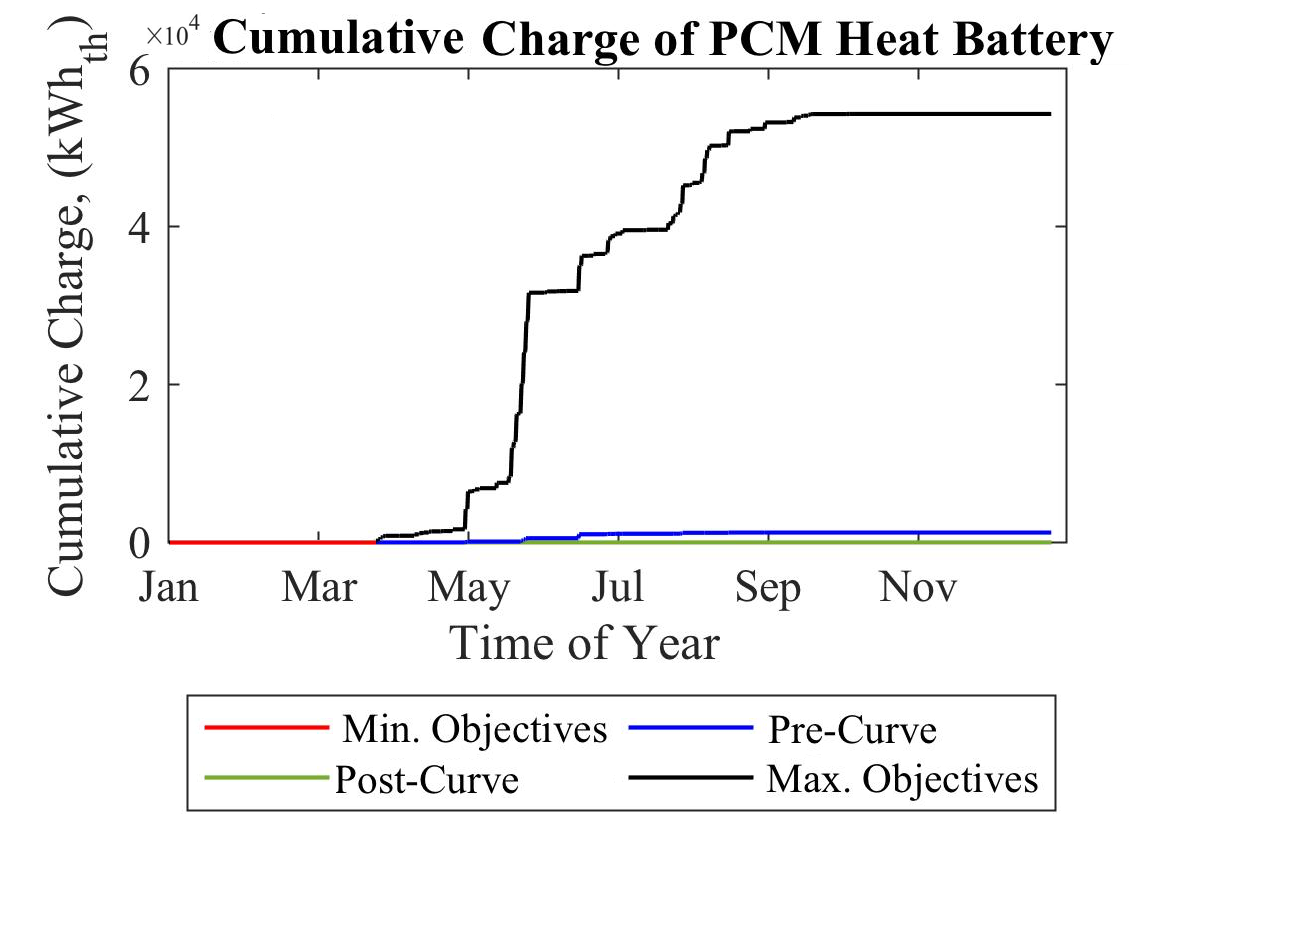
\includegraphics[width=255pt]{Figures/CumChargeHBat.png}
    \vspace*{-15mm}
    \caption{Four scenarios for the cumulative charge of the PCM heat battery array with respect to time. Each line represents one point on the Pareto front from lowest consumer cost to highest consumer cost.}
    \label{fig:CumChargeHBat}
\end{figure}

Fig. \ref{fig:CumChargeBat} and Fig. \ref{fig:CumChargeHBat} show the cumulative charge of the Li-Ion battery array and PCM heat battery array with respect to time. For both, the best scenario is when the maximum consumer cost solution is used. This is due to a higher amount of panels and batteries being used in this case and as such, more energy is generated and stored. The Li-Ion battery array reaches its highest cumulative point at 2 GWh in the highest consumer cost scenario. At minimum consumer cost, the storage is almost zero throughout the simulation as there is minimal storage capacity on site. Similarly for the PCM heat battery array, three of the four scenarios indicate minimal thermal energy storage. The best case peaks at 54 MWh of cumulative storage.

\subsubsection{Areal Coverage}
\vspace*{1mm}
\begin{figure}[H]
	\centering
    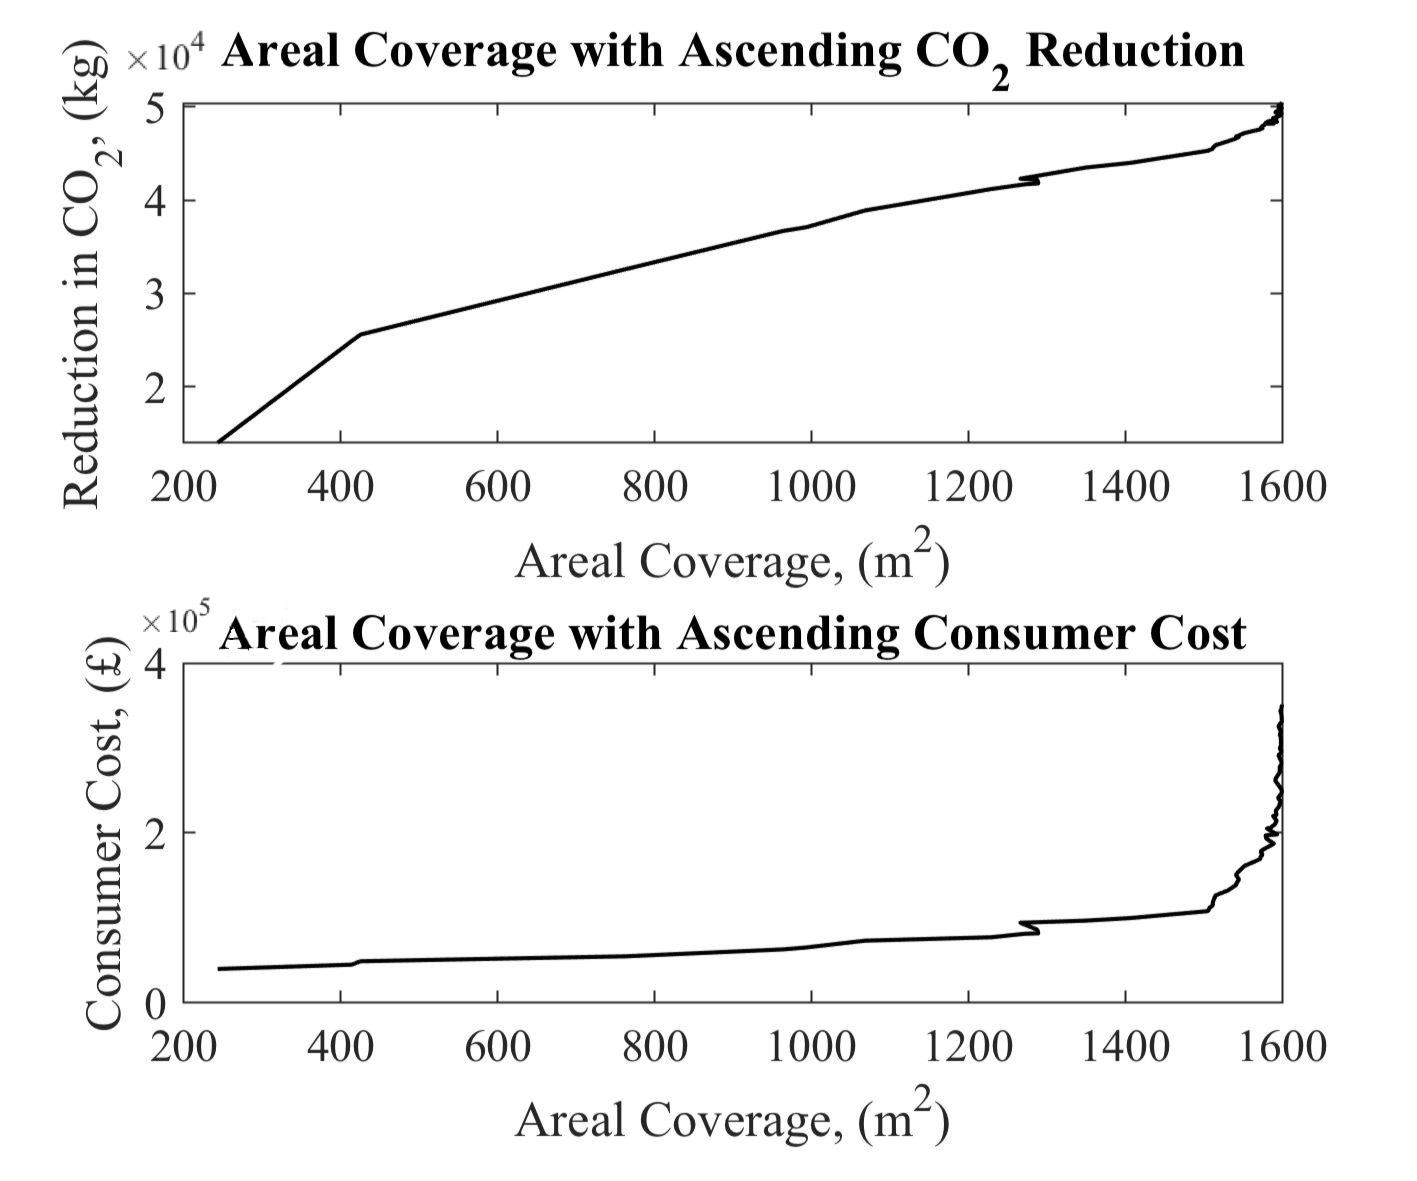
\includegraphics[width=245pt]{Figures/ArealCoverage.jpg}
    \caption{Areal coverage of panels on roof space with respect to the two objective functions.}
    \label{fig:ArealCoverage}
\end{figure}

Fig. \ref{fig:ArealCoverage} indicates that the higher the value of the objective functions is, the more areal space is covered by panels. The top graph indicates a reasonably steady climb in CO$_2$ reduction with an increase in areal coverage. The bottom graph has a steady inclination in consumer cost up until around 1500m$^2$, where there is a sharp increase in the consumer cost for a relatively small increase in areal coverage. This indicates that at higher areal coverage, a larger amount of storage is required and thus a large spend on batteries is required. It is also noticeable that the maximum area of 1600m$^2$ is not exceeded and therefore the constraint on the number of panels allowed (or maximum area allowed) is limiting the solution space as intended.

\subsubsection{Sensitivity Analysis}

Sensitivity analysis is performed on the Pareto front by altering the demand from the base case to 50\% and 10\%.

\begin{figure}[H]
	\centering
    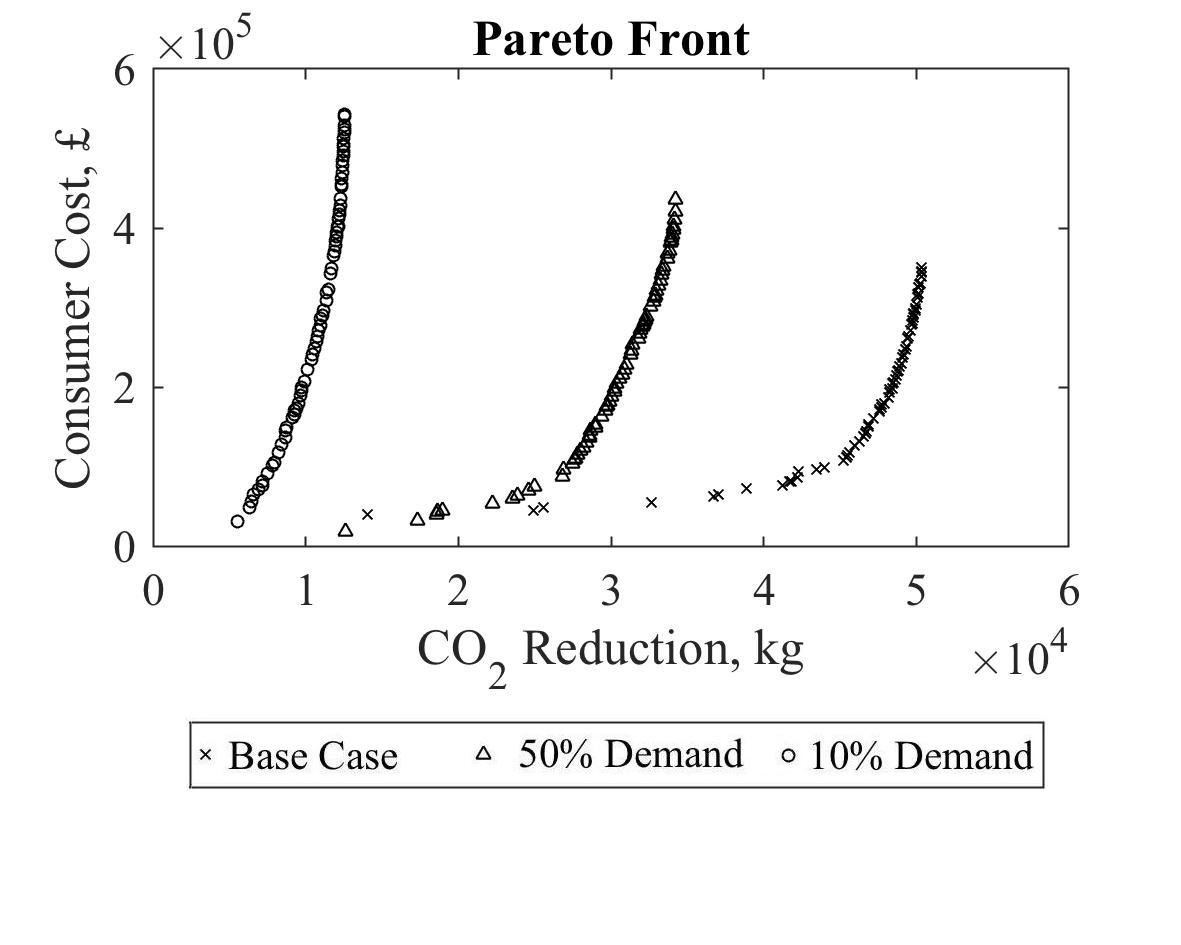
\includegraphics[width=\columnwidth]{Figures/ParetoSens1.jpg}
    \vspace*{-15mm}
    \caption{Sensitivity of the Pareto front to change in the electrical and thermal energy demand. Base case, 50\% and 10\% demand scenarios are shown.}
    \label{fig:ParetoSens}
\end{figure}
  
Fig. \ref{fig:ParetoSens} shows the effect of varying the demand on the Pareto front. The base case, indicated by X shows the same data as was described previously. When the demand is halved, the Pareto front shifts to the right. The trend is very similar to the base case and therefore the system is reasonably robust. However, when the demand is cut to just 10\%, the Pareto front shifts greatly to the right and the curve is different in shape. It transitions more smoothly and gradually than that of the base case and halved demand case. The difference is most evident in the middle of the curve where it is greatly different. This indicates that the system can handle small changes in the demand but would become inaccurate if the demand is greatly changed from the values it is designed for.

\subsection{Case 2: Australia}

Case 1 uses the Lord Thomson building at Heriot-Watt University as the demand. The resource data used is for Perth, Australia. Three scenarios are simulated which include the base case, where the demand is unchanged, a reduced demand scenario, where the demand is reduced by 20\% and an increased demand scenario where the demand is increased by 20\%.  This case allows for results to be seen where solar-thermal is a viable solution.

\subsubsection{Pareto Front}

\begin{figure}[H]
	\centering
    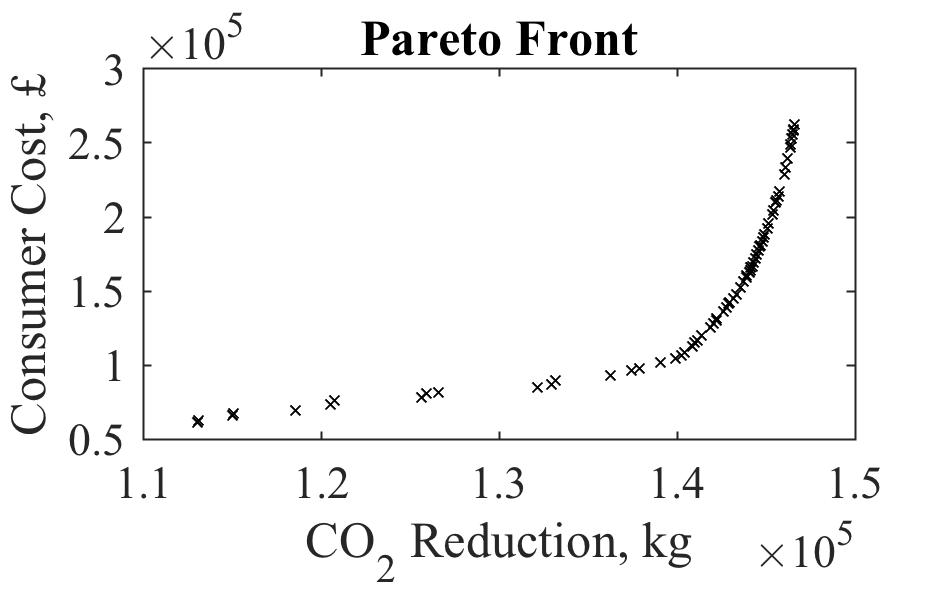
\includegraphics[width=0.95\columnwidth]{Figures/ParetoFront2.jpg}
    \caption{The Pareto front for the case 2 base scenario. The two optimised objective functions are plotted with consumer cost on the y-axis and CO$_2$ reduction on the x-axis.}
    \label{fig:ParetoFront2}
\end{figure}

Fig. \ref{fig:ParetoFront2} shows the Pareto front obtained from the simulation of case 2. The range of solutions is from £60,000 to £250,000. The CO$_2$ reduction ranges from approximately 105,000 to 145,000 kg. In this case, the constraint on the minimum acceptable solution is set to 50\% of the total demand. Since the resource has been changed, the amount of energy generated can be greatly increased, thus allowing for a more limiting constraint which results in a smaller range in the solution. The reduction in CO$_2$ starts much higher than that of case 1 as there is a larger solar radiation available and less allowance for variance in the number of panels due to the constraint of meeting 50\% of the total demand.

\begin{table}[H]
\caption{Four selected solutions on the Pareto front ranging from minimum to maximum points for Case 2.}
\vspace{5pt}
\label{case2}
\centering
\begin{tabular}{@{}llll@{}}
\toprule
\begin{tabular}{@{}l@{}}{\textbf{CO$_2$}} \\ \textbf{Reduction, kg}\end{tabular} 
& \begin{tabular}{@{}l@{}}{\textbf{Consumer}} \\ \textbf{Cost, £}\end{tabular} 
& \begin{tabular}{@{}l@{}}{\textbf{PV/ST}}  \\ \textbf{Panels}\end{tabular}
& \begin{tabular}{@{}l@{}}{\textbf{Li-ion/Heat}} \\ \textbf{Batteries}\end{tabular} \\ \toprule
147,000 & 262,000 & 253/441 & 51/38 \\ \midrule
143,000 & 147,000 & 382/315 & 26/38 \\ \midrule
133,000 & 90,000 & 440/259 & 13/36 \\ \midrule
113,000 & 61,500 & 456/245 & 2/35 \\ \midrule
\end{tabular}
\end{table}

Table \ref{case2} gives four selected solutions on the Pareto front. These solutions range from the maximum to minimum points on the pareto front. Each is an optimised solution to the problem which lies on the front.

\subsubsection{Optimised Objectives vs Simulation Variables}

\begin{figure}[H]
	\centering
    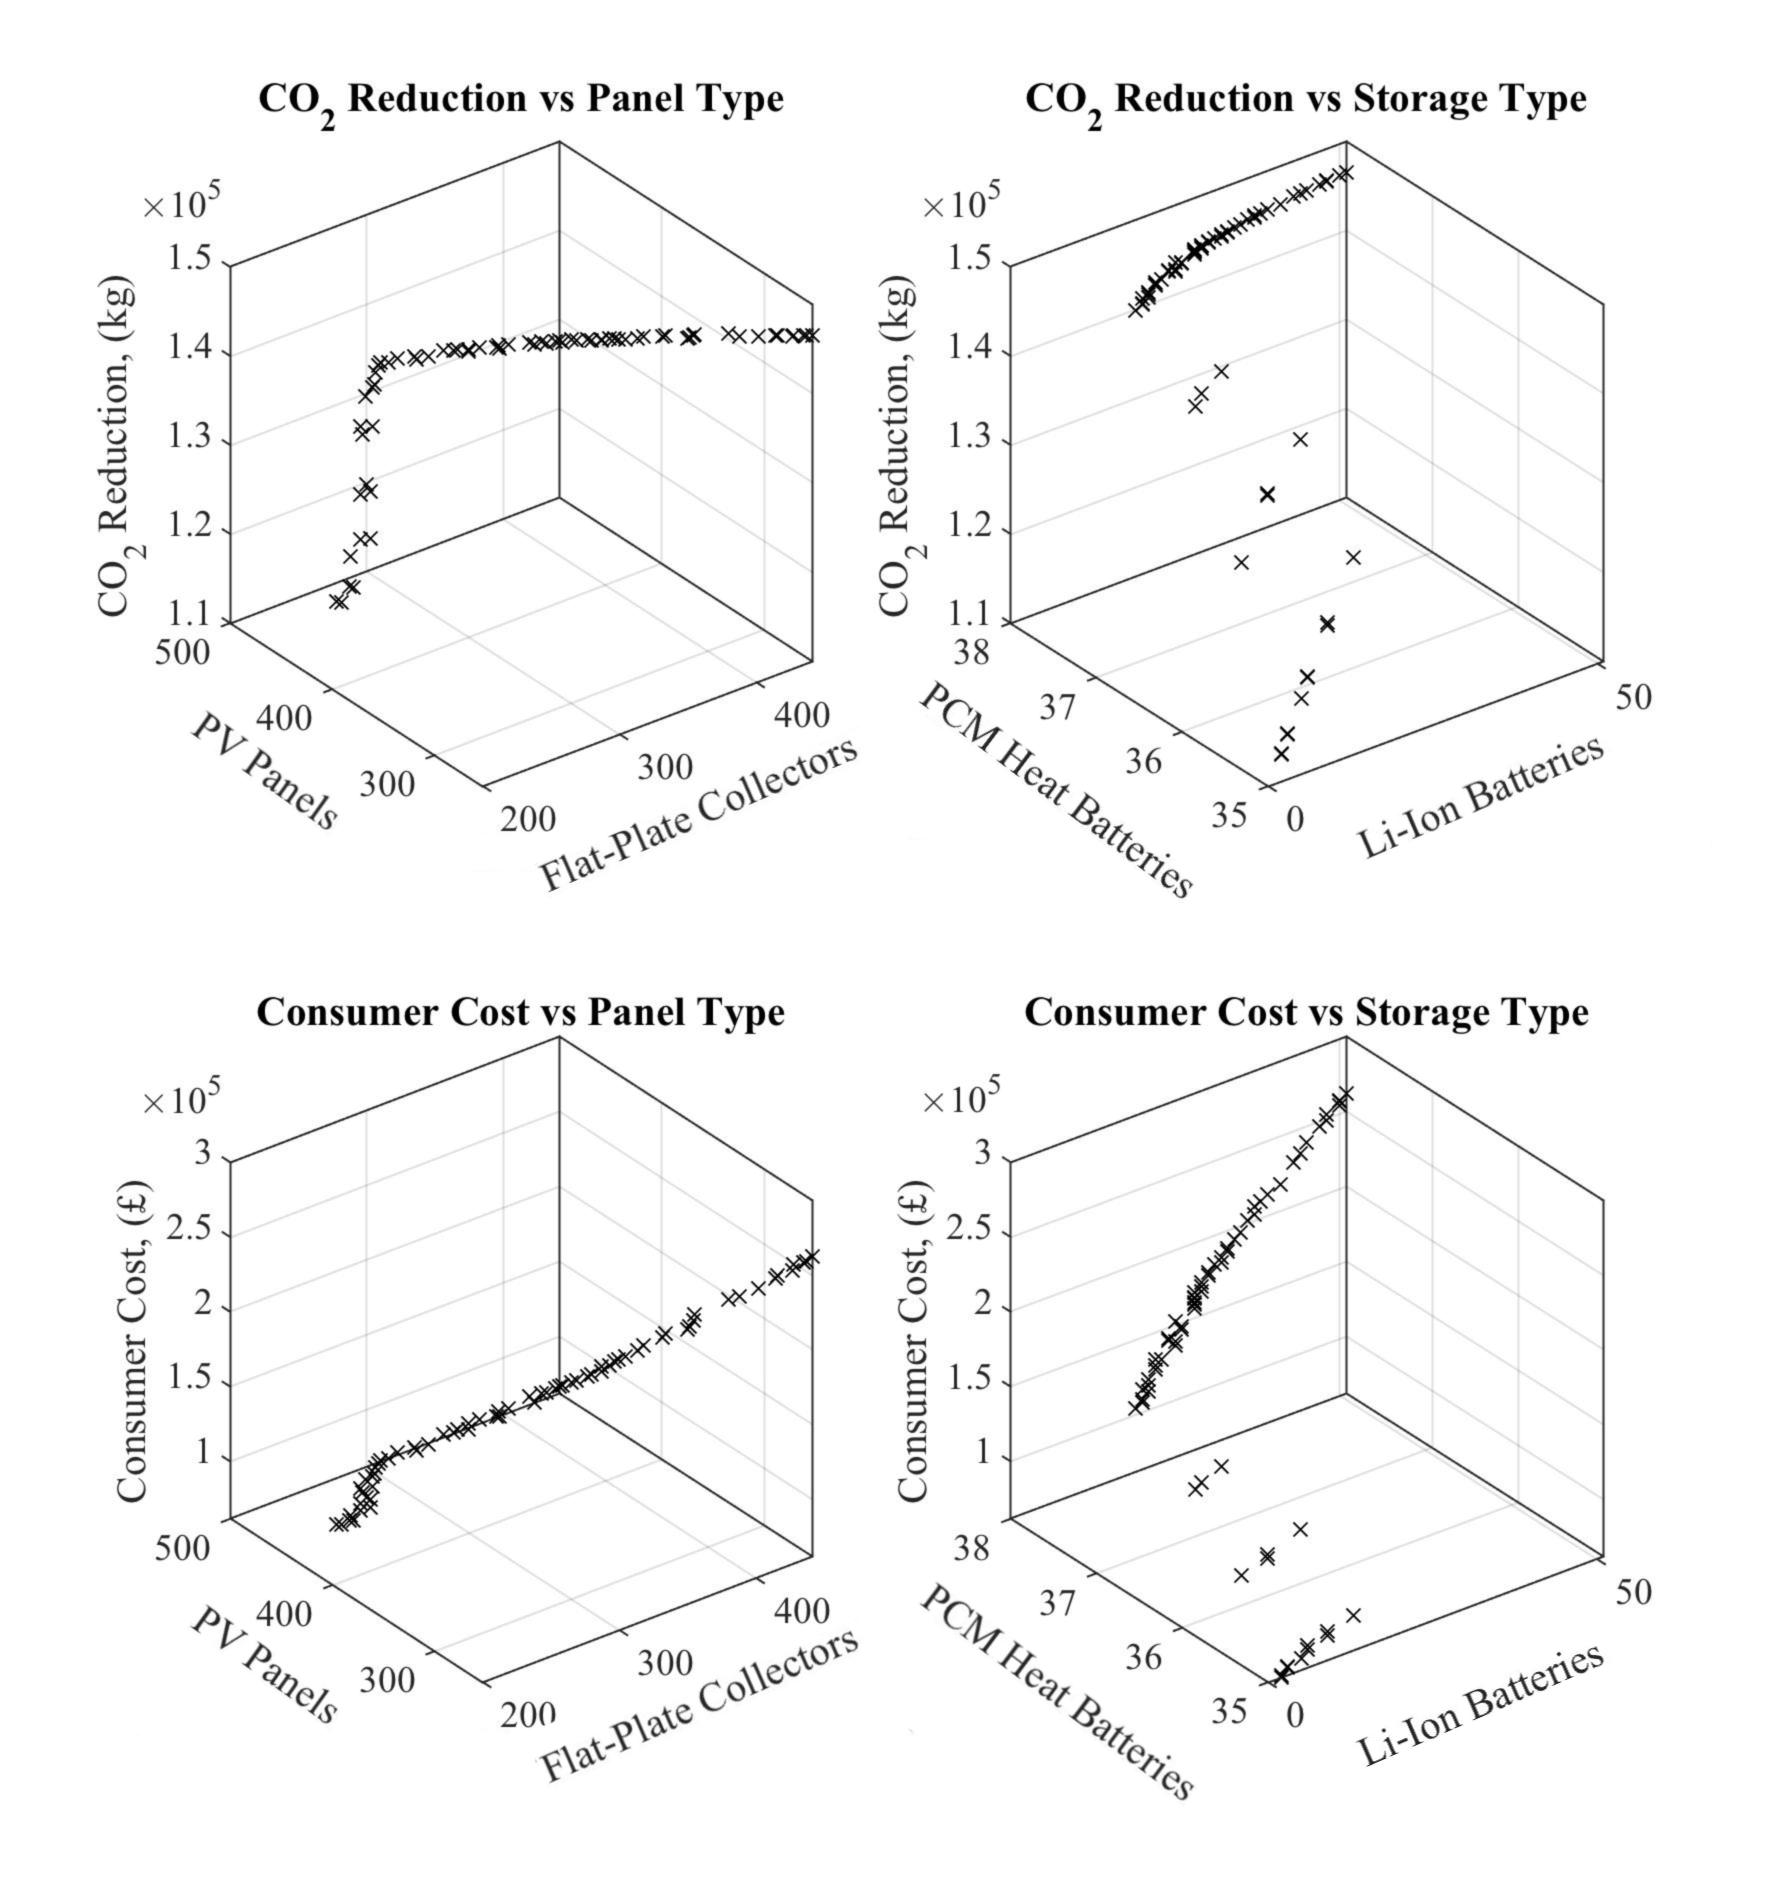
\includegraphics[width=\columnwidth]{Figures/RedAndCostVsPanelsAndStorage2.jpg}
    \caption{3-Dimensional plots of the optimised objectives with respect to the the simulation variables. (a) Panel type vs CO$_2$ reduction, (b) Storage type vs CO$_2$ reduction, (c) Panel type vs consumer cost, and (d) Storage type vs consumer cost}
    \label{fig:ObjectivesVsPanelsVsStorage2}
\end{figure}

Fig. \ref{fig:ObjectivesVsPanelsVsStorage2} shows the reduction in CO$_2$ emissions with respect to PV panels and flat plate collectors. The number of panels is more restricted in this case and varies from 300-500 and 250-450 for PV and flat-plate collectors respectively. The highest reduction in CO$_2$ emissions (approximately 145,000 kg) is present when the number of flat-plate collectors is maximised. Similarly, Fig. \ref{fig:ObjectivesVsPanelsVsStorage2}(c) shows the consumer cost with respect to the number of PV panels and flat plate collectors respectively. The trend is very similar to that of the CO$_2$ reduction, indicating that the consumer cost will peak at a higher ratio of flat plate collectors to PV panels. However, as the amount of PV panels is increased, the consumer cost is reduced. This is due to the generation tariff on PV panels. In reality, this tariff and resource would not occur together. Fig. \ref{fig:ObjectivesVsPanelsVsStorage2}(b) and Fig. \ref{fig:ObjectivesVsPanelsVsStorage2}(d) show the CO$_2$ reduction and consumer cost with respect to each storage method. The simulation is heavily weighted towards a set amount of PCM heat batteries as in order to meet the demand, this storage method is required in large quantities. The variation in Li-Ion batteries is from 0-50, indicating more leniency in electricity storage. It can be seen that as the amount of batteries in the system increases, the consumer cost will increase. Similarly, The CO$_2$ reduction generally increases with the amount of batteries. However, this is due to the increased generation (thus increased reduction in emissions) and not due to the amount of batteries in the system.
  
\subsubsection{Storage Performance}

\begin{figure}[H]
	\centering
    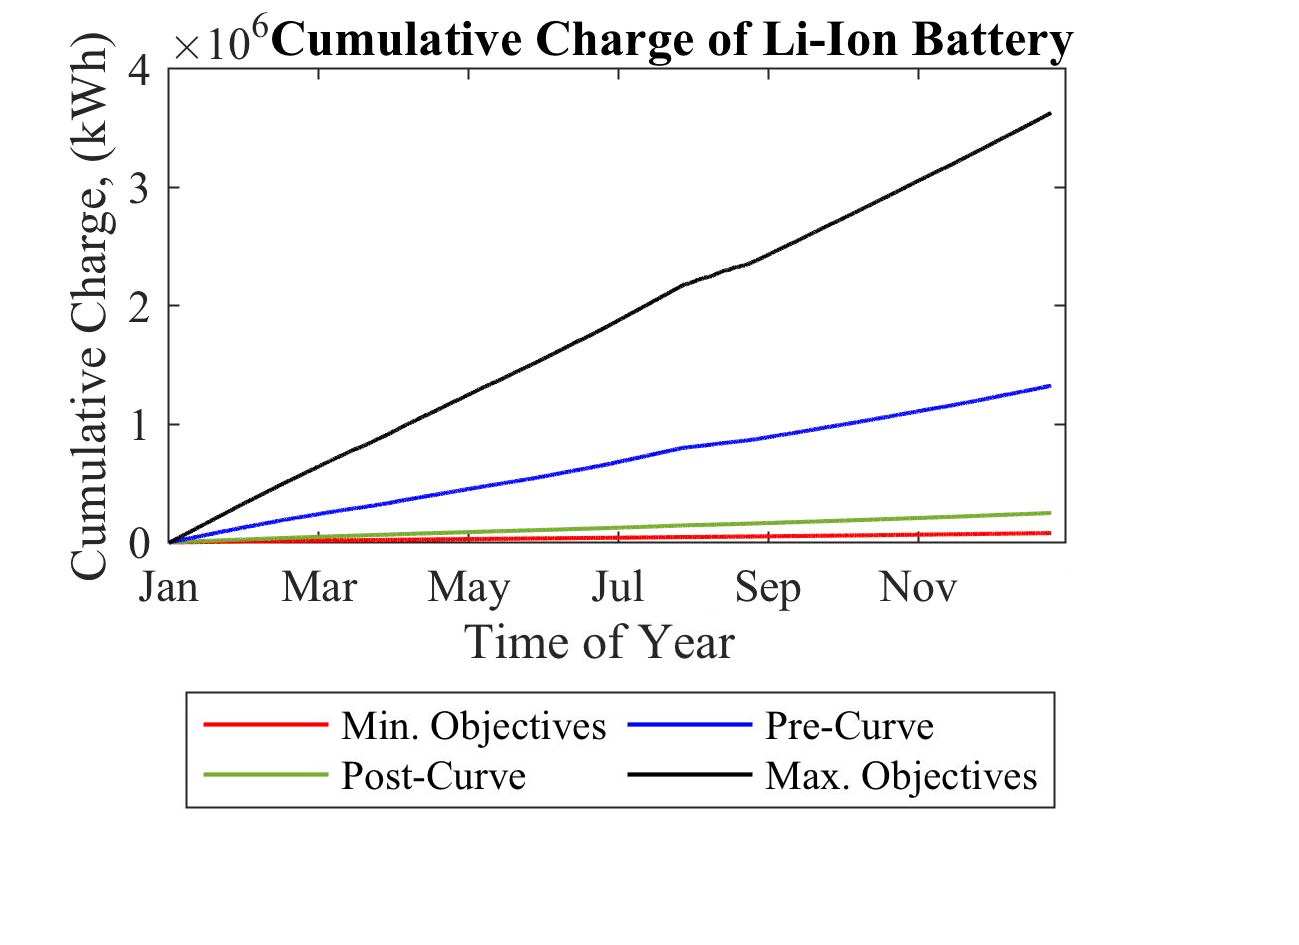
\includegraphics[width=1.12\columnwidth]{Figures/CumBat2.png}
    \caption{Four scenarios for the cumulative charge of the Li-Ion battery array with respect to time. Each line represents one point on the Pareto front from lowest consumer cost to highest consumer cost.}
    \label{fig:CumBat2}
\end{figure}
 
 \begin{figure}[H]
	\centering
    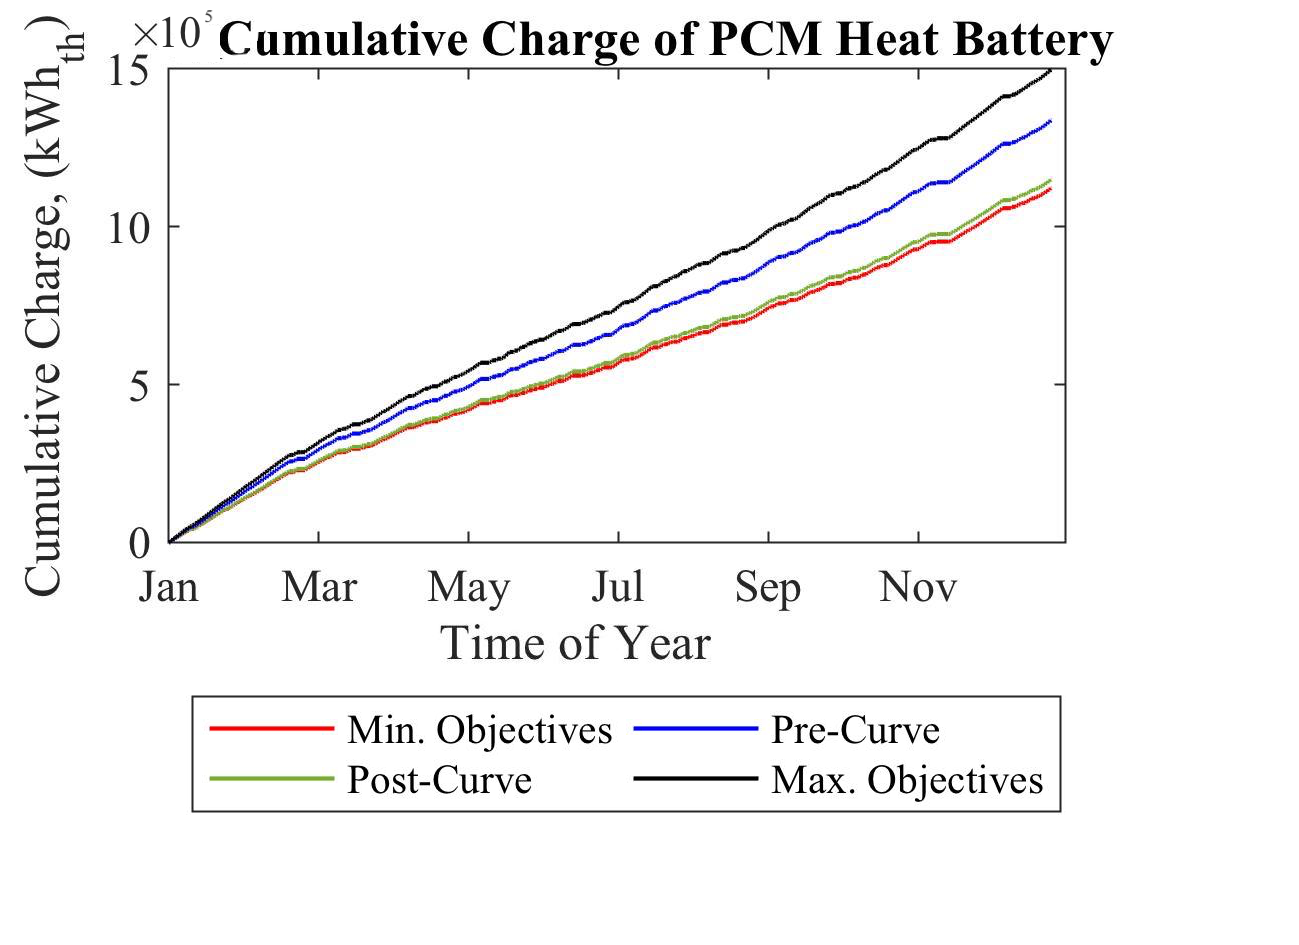
\includegraphics[width=1.12\columnwidth]{Figures/CumHBat2.png}
    \caption{Four scenarios for the cumulative charge of the PCM heat battery array with respect to time. Each line represents one point on the Pareto front from lowest consumer cost to highest consumer cost.}
    \label{fig:CumHBat2}
\end{figure}


Fig. \ref{fig:CumBat2} and Fig. \ref{fig:CumHBat2} show the cumulative charge of the battery arrays for both electrical and thermal storage. In this case, the same trend as case 1 is shown in that as the consumer cost is increased (and reduction in CO$_2$ is also increased) the performance of the storage is also increased. For the Li-Ion battery array, 
the cumulative charge reaches a maximum level of 3.5 GWh and the PCM heat battery array reaches 1.5 GWh of thermal storage. All four scenarios for the PCM heat battery increase linearly throughout the year and even in the case of the lowest consumer cost scenario, there is still a cumulative charge of 1 GWh thermal energy stored. This indicates that when there is a high solar radiation present, the simulation will lean towards maximising the solar thermal potential. In both types of storage, the maximum is higher than that of case 1.

\subsubsection{Areal Coverage}

\begin{figure}[H]
	\centering
    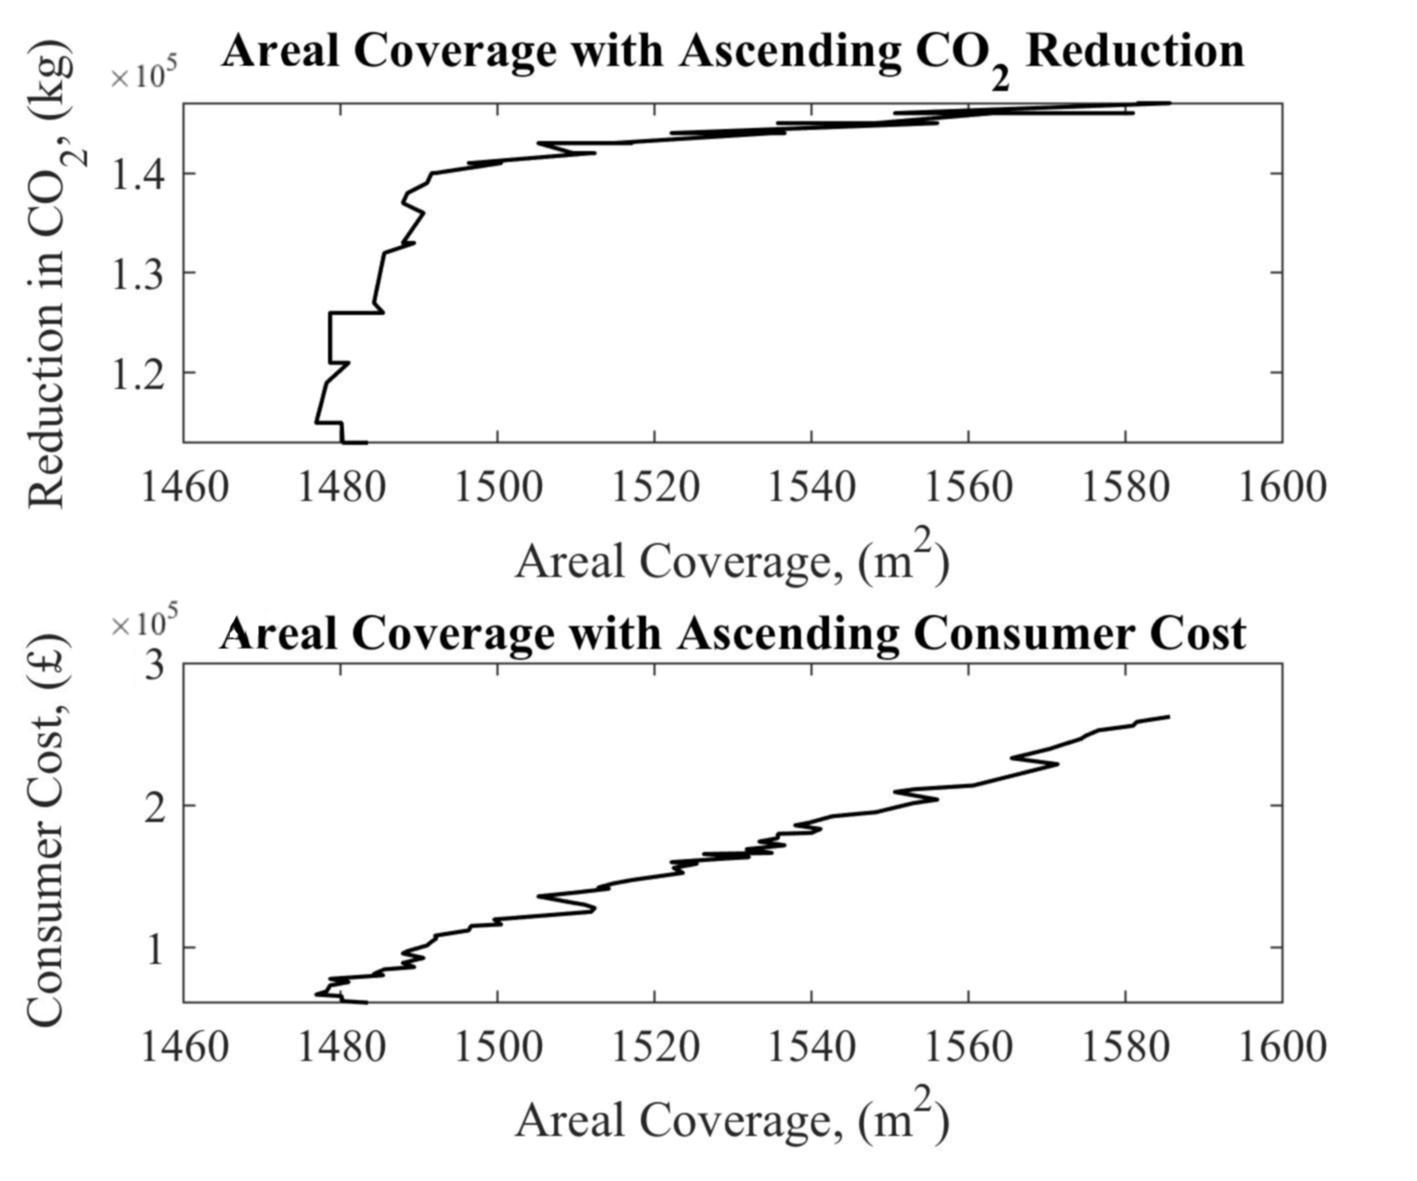
\includegraphics[width=\columnwidth]{Figures/ArealCoverage2.jpg}
    \caption{Areal coverage of panels on roof space with respect to the two objective functions for case 2}
    \label{fig:ArealCoverage2}
\end{figure}

Fig. \ref{fig:ArealCoverage2} indicates that the higher the value of the objective functions is, the more areal space is covered by panels. This trend is visible but in this case there is much more variation. The areal coverage covers a much shorter range of areas for case 2. This is due to the demand constraint meaning a minimum area of around 1480m$^2$ being required. Since the range is smaller, the small changes in the two objective functions are more noticeable. However, the trends are still similar in nature to that of case 1. The jagged nature of the line in the lower graph indicates that despite an increase in the consumer cost, the areal coverage can go down. This is due to the increased amount of storage being used in order to meet the requirements. The maximum area of 1600m$^2$ is not reached for this case as it peaks at 1585m$^2$. This 15m of remaining areal space would only be able to include approximately 7 panels of either type and therefore does not impact the result greatly.
  
\subsubsection{Sensitivity Analysis}

\begin{figure}[H]
	\centering
    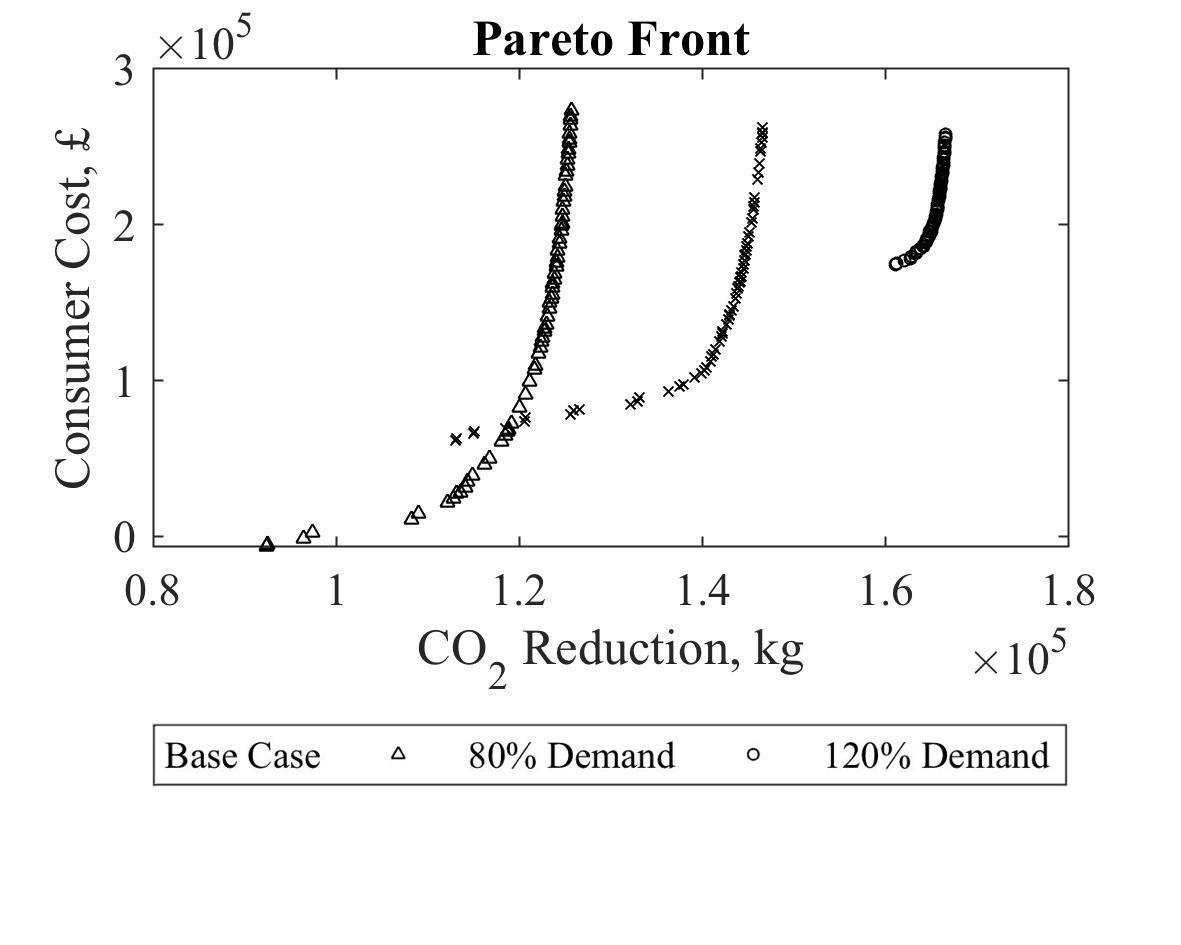
\includegraphics[width=\columnwidth]{Figures/ParetoSens2.jpg}
    \caption{Sensitivity of the Pareto front to change in the electrical and thermal energy demand. Base case, +20\% and -20\% demand scenarios are shown.}
    \label{fig:ParetoSens2}
\end{figure}

Fig. \ref{fig:ParetoSens2} shows the sensitivity of the Pareto front for case 2 when the demand is varied. In this case, the demand has been varied +/- 20\%. It is evident that this change in demand has a large effect on the curve. An increase in the demand of 20\% shifts the curve to the left. It also curves round much earlier than that of the base case, indicating that in this scenario, the solution is not robust. Similarly, a decrease in the demand of 20\% shifts the curve to the right. The spread of solutions is much wider in this case as the program has more room to change. This results in a smoother transition in the curve. In summary, it can be stated that any change in the demand will greatly affect where optimal solutions lie, and therefore use of the model in practice should be limited to scenarios in which there is a high confidence in the demand, resource and other contributing factors.

